\documentclass[conference]{IEEEtran}
\usepackage[T1]{fontenc}
\usepackage{graphicx}
\usepackage{booktabs}
\usepackage{amsmath,amssymb}
\usepackage{siunitx}
\usepackage{xcolor}
\usepackage{url}
\usepackage[hidelinks]{hyperref}
\sisetup{detect-all, group-minimum-digits=4}
\graphicspath{{../../results/}{../../slides/figures/}{../figures/}{figures/}}
\newcommand{\pp}{\,pp}
\raggedbottom  % no stretched gap between a float and the text below it

\begin{document}

\title{98\,\% Accuracy Holds on Unseen Patients: A Code-Exact Reproduction and Pre-Registered Patient-Level Ablation of an EfficientNet-B0 Malaria Ensemble}

\author{
\IEEEauthorblockN{J Amathziah (230139), C Murali Madhav (230115), Ravi Yadav (230131), Pugazhendhi J (230066)}
\IEEEauthorblockA{Department of Computer Science, Rishihood University, Sonipat, India\\
Code, results and trained models: \url{https://github.com/amathziah/malaria-detection}}
}

\maketitle

\begin{abstract}
Deep-learning studies on the NIH malaria cell images report 96 to 99.9\,\% accuracy, almost always with random image-level splits that place cells of the same patient in both the training and the test set. We rebuild the EfficientNet-B0 ten-fold ensemble of Marques \emph{et al.}\ (2022) exactly from the authors' executed code and test, in a pre-registered ablation, whether its accuracy holds on unseen patients and whether YUV histogram-equalisation stain normalisation adds anything there.
The reproduction matches the paper within 1 percentage point (pp) on every metric (mean fold accuracy 97.55 vs.\ 97.56\,\%), is verified by 32 automated tests, trains about 25 times faster, and corrects three reporting errors.
On 40 patients held out entirely, the ensemble reaches 98.45\,\% accuracy (95\,\% patient-bootstrap CI 97.94 to 98.91\,\%), 98.05\,\% recall and 99.80\,\% ROC-AUC, on par with the paper's 98.29\,\% on a random split. Measured on \num{17591} identical cells, patient leakage is small: 0.85\,pp of Matthews correlation (MCC; 95\,\% CI 0.05 to 2.02).
YUV normalisation is equivalent to no preprocessing within $\pm$1\,pp of MCC (90\,\% CI $-0.73$ to $+0.16$; TOST $p=0.008$), so the simpler pipeline loses nothing. In an exploratory patient-level analysis, a rule chosen without the test patients identifies 26 of 28 infected and all 12 healthy held-out patients. All 40 models, the code and the analysis plan are public.
\end{abstract}

\begin{IEEEkeywords}
malaria, thin blood smear, EfficientNet, ensemble learning, reproducibility, data leakage, patient-level validation, stain normalisation
\end{IEEEkeywords}

\section{Introduction}
Malaria is diagnosed by examining Giemsa-stained blood smears under a microscope, where a trained technician inspects red blood cells for parasites. The method is the clinical gold standard, but it is slow, it depends on scarce expertise in exactly the regions where malaria is common, and its results vary between observers and laboratories. Automated classification of single red-blood-cell images is therefore an active research topic, and on the public NIH Malaria Cell Images dataset~\cite{rajaraman2018} convolutional neural networks (CNNs) routinely report accuracies of 96 to 99.9\,\%~\cite{liang2016,rajaraman2018,rajaraman2019,umer2020,fuhad2020,zhao2020,masud2020,marques2022,madhu2023,hemachandran2023,mujahid2024}.

Two questions decide whether such numbers can be trusted. First, \emph{can they be reproduced?} Papers rarely publish their full training code, and small undocumented choices (augmentation, label smoothing, checkpointing) move the results by more than the differences being claimed. Second, \emph{do they hold on patients the model has never seen?} Most studies split the 27{,}558 cell images at random, so cells of the same patient, which share stain, illumination and the patient's own blood, appear in both the training and the test set. A model could then score well by recognising the patient rather than the parasite.

We answer both questions for a strong, openly documented baseline: the EfficientNet-B0 ten-fold ensemble of Marques \emph{et al.}~\cite{marques2022}, whose authors published their executed notebook. Our contributions are:
\begin{enumerate}
\item \textbf{A code-exact reproduction, 25 times faster.} Built from the authors' notebook and verified by 32 tests against the paper's printed outputs, it matches every metric within 1\,pp and trains a fold in about 11 minutes instead of 4\,h\,46\,min. It also corrects three reporting errors: swapped precision and recall, randomly augmented evaluation images, and a table that reports $(\text{precision}+\text{recall})/2$ as accuracy.
\item \textbf{Accuracy that holds on unseen patients:} 98.45\,\% accuracy, 98.05\,\% recall and 99.80\,\% ROC-AUC on 40 patients the models never saw, on par with the paper's random-split result.
\item \textbf{Patient leakage measured, not assumed:} 0.85\,pp of MCC on \num{17591} identical cells scored by models that had and had not seen each patient.
\item \textbf{Stain normalisation shown to be unnecessary:} YUV histogram equalisation~\cite{umer2020} is equivalent to no preprocessing within $\pm$1\,pp of MCC on unseen patients.
\item \textbf{A rigorous, open protocol:} hypotheses, decision rules and metric committed before training; patient-level bootstrap intervals, corrected resampled $t$-tests~\cite{nadeau2003} and Holm correction~\cite{holm1979}; exploratory analyses fixed in a dated addendum before they were run; all 40 models and the code public.
\end{enumerate}

\section{Related Work}
Liang \emph{et al.}~\cite{liang2016} showed that a 16-layer CNN trained from scratch (97.37\,\%) outperforms transferred AlexNet features (91.99\,\%). Rajaraman \emph{et al.}~\cite{rajaraman2018} released the NIH dataset and mapped which layers of pre-trained CNNs transfer best; importantly, they evaluated at the patient level as well as the cell level and observed lower scores at the patient level. Ensembles followed: Rajaraman \emph{et al.}~\cite{rajaraman2019} combined VGG-19 and SqueezeNet, and Marques \emph{et al.}~\cite{marques2022} averaged ten EfficientNet-B0 models from a ten-fold cross-validation (98.29\,\% accuracy, ROC-AUC 99.76\,\%). Lightweight models target point-of-care use: Fuhad \emph{et al.}~\cite{fuhad2020} reached 99.23\,\% with about 4{,}600 FLOPs on a phone after cleaning the dataset's labels, and Masud \emph{et al.}~\cite{masud2020} used a 409\,K-parameter CNN. Zhao \emph{et al.}~\cite{zhao2020} extended detection to a second species. Umer \emph{et al.}~\cite{umer2020} preprocessed images by YUV conversion and luma histogram equalisation before a stacked CNN and reported $\sim$99.9\,\%. Capsule networks~\cite{madhu2023} and systematic backbone comparisons~\cite{hemachandran2023,mujahid2024} complete the picture.

Two gaps run through this literature. Protocols differ (5-fold, 10-fold and 80:20 splits; original or cleaned labels), so reported accuracies are not directly comparable. And most studies split images at random, so the same patient's cells sit on both sides of the split; only Rajaraman \emph{et al.}~\cite{rajaraman2018,rajaraman2019} report patient-level evaluation. We take the strongest reproducible baseline and measure, with a pre-registered protocol, how much of its accuracy holds on unseen patients.

\section{Data}
The NIH Malaria Cell Images dataset~\cite{rajaraman2018} contains \num{27558} segmented single-cell crops (\num{13779} parasitized, \num{13779} uninfected) from Giemsa-stained thin smears of 200 patients (150 infected with \emph{P.~falciparum}, 50 healthy), photographed through a microscope with a smartphone at Chittagong Medical College Hospital, Bangladesh. Crops vary in size and are resized to $224\times224$.

\textbf{Patient identity.} Every file name begins with the patient's case number, e.g.\ \path{C33P1thinF_IMG_..._cell_179.png} belongs to patient C33. We verified this key against NIH's own patient-to-cell mapping files: all \num{27558} cells map, giving 200 patients. NIH lists one patient (C47) under two keys, one per microscope; the case number correctly merges them. Infected patients also contribute uninfected cells: \num{10364} of the \num{13779} uninfected cells come from infected patients' smears. Under a random split, almost every patient therefore has cells on both sides. Patients differ widely: 65 to 702 cells each, and 1 to 90\,\% parasitized among the infected.

\section{Methods}
\subsection{Code-exact reproduction of the baseline (A0)}
The supplementary file of~\cite{marques2022} is the authors' executed notebook. It differs from the paper's text in several respects, and we follow the code: noisy-student EfficientNet-B0 weights~\cite{tan2019,xie2020} (qubvel \texttt{efficientnet} 1.1.1, all layers trainable) followed by global average pooling and dense layers of 128, 64 and 32 units (ReLU, dropout 0.3) and a two-way softmax; categorical cross-entropy with label smoothing 0.1; Adam (learning rate $10^{-4}$); learning-rate halving on a validation-loss plateau (patience 6, minimum $10^{-6}$); 33 epochs of batch size 16 with the best-validation-loss weights restored; and a heavy \texttt{albumentations} pipeline (flips, $90^\circ$ rotations, noise, blur, shift-scale-rotate, optical, grid and piecewise-affine distortions, CLAHE, sharpening, embossing, contrast and brightness changes). The data are split 80/20 into a learning set and an untouched hold-out set; a stratified ten-fold cross-validation on the learning set yields ten models, and the ensemble averages their softmax outputs on the hold-out set.

We reimplemented this recipe in TensorFlow~2.15 with the same Keras~2 API and library versions, and wrote 32 tests that compare it with the paper: the parameter counts of its Table~2 (\num{4223934} total, \num{4181918} trainable), the split and fold sizes printed by its code, the exact augmentation pipeline, image loading identical to the authors' generator, the loss, optimiser and callbacks, and its classification reports. The paper's split was unseeded and cannot be recovered; we sort the file list and seed the split so that every machine builds the same one, and store a fingerprint of the split with every fold.

\textbf{Speed without changing the computation.} Images are decoded once into a shared \texttt{uint8} array; the augmentation runs in worker processes, each batch seeded by (fold, epoch, batch) so results do not depend on the number of workers; batches reach the GPU as \texttt{uint8} and are scaled inside the model; and the training step is XLA-compiled. Arithmetic remains float32. Each fold trains on its own RTX~4090 in about 11 minutes, against 4\,h\,46\,min per fold reported for a GTX~1050.

\subsection{Ablation design (A1 to A3)}
Each experiment changes one thing relative to A0 (Table~\ref{tab:design}); everything else, including the per-fold seeds, is identical. H1 predicts that random splits inflate the scores; H2, that YUV normalisation helps on unseen patients.

\begin{table}[t]
\centering
\caption{Ablation design. Every experiment uses A0's recipe and ten folds.}
\label{tab:design}
\begin{tabular}{@{}llll@{}}
\toprule
ID & Split & Preprocessing & Question \\
\midrule
A0 & image (paper) & none & baseline \\
A1 & patient & none & H1: leakage (A1 vs A0) \\
A2 & patient & YUV + hist.-eq. & H2: normalisation (A2 vs A1) \\
A3 & image (paper) & YUV + hist.-eq. & control (A3 vs A0) \\
\bottomrule
\end{tabular}
\end{table}

\textbf{Patient split (A1, A2).} \texttt{StratifiedGroupKFold} with five groups proposes five hold-out sets of about 20\,\% of the cells; we take the one closest to 20\,\% of the cells and 50\,\% parasitized, a rule on labels only. This yields \num{5550} hold-out cells from 40 patients (28 infected; 50.7\,\% parasitized). The remaining 160 patients are split into ten folds of 15 to 17 patients by \texttt{StratifiedGroupKFold}. The split is committed to the repository and every training run verifies its fingerprint; A1 and A2 use the identical split, and A3 reuses A0's split exactly, so both pairs compare the same cells fold by fold.

\textbf{YUV normalisation (A2, A3).} Following~\cite{umer2020}, each image is converted to YUV, the luma channel is histogram-equalised, and the result is converted back to RGB, at the image's native size and before the unchanged resize and augmentation. Chroma is untouched and the black background stays black. We omit the 120\,$\times$\,120 resize and the unspecified edge kernel of~\cite{umer2020}. Fig.~\ref{fig:yuv} shows the effect: the narrow brightness range of each cell is stretched over the full range, which also amplifies texture.

\begin{figure*}[t]
\centering
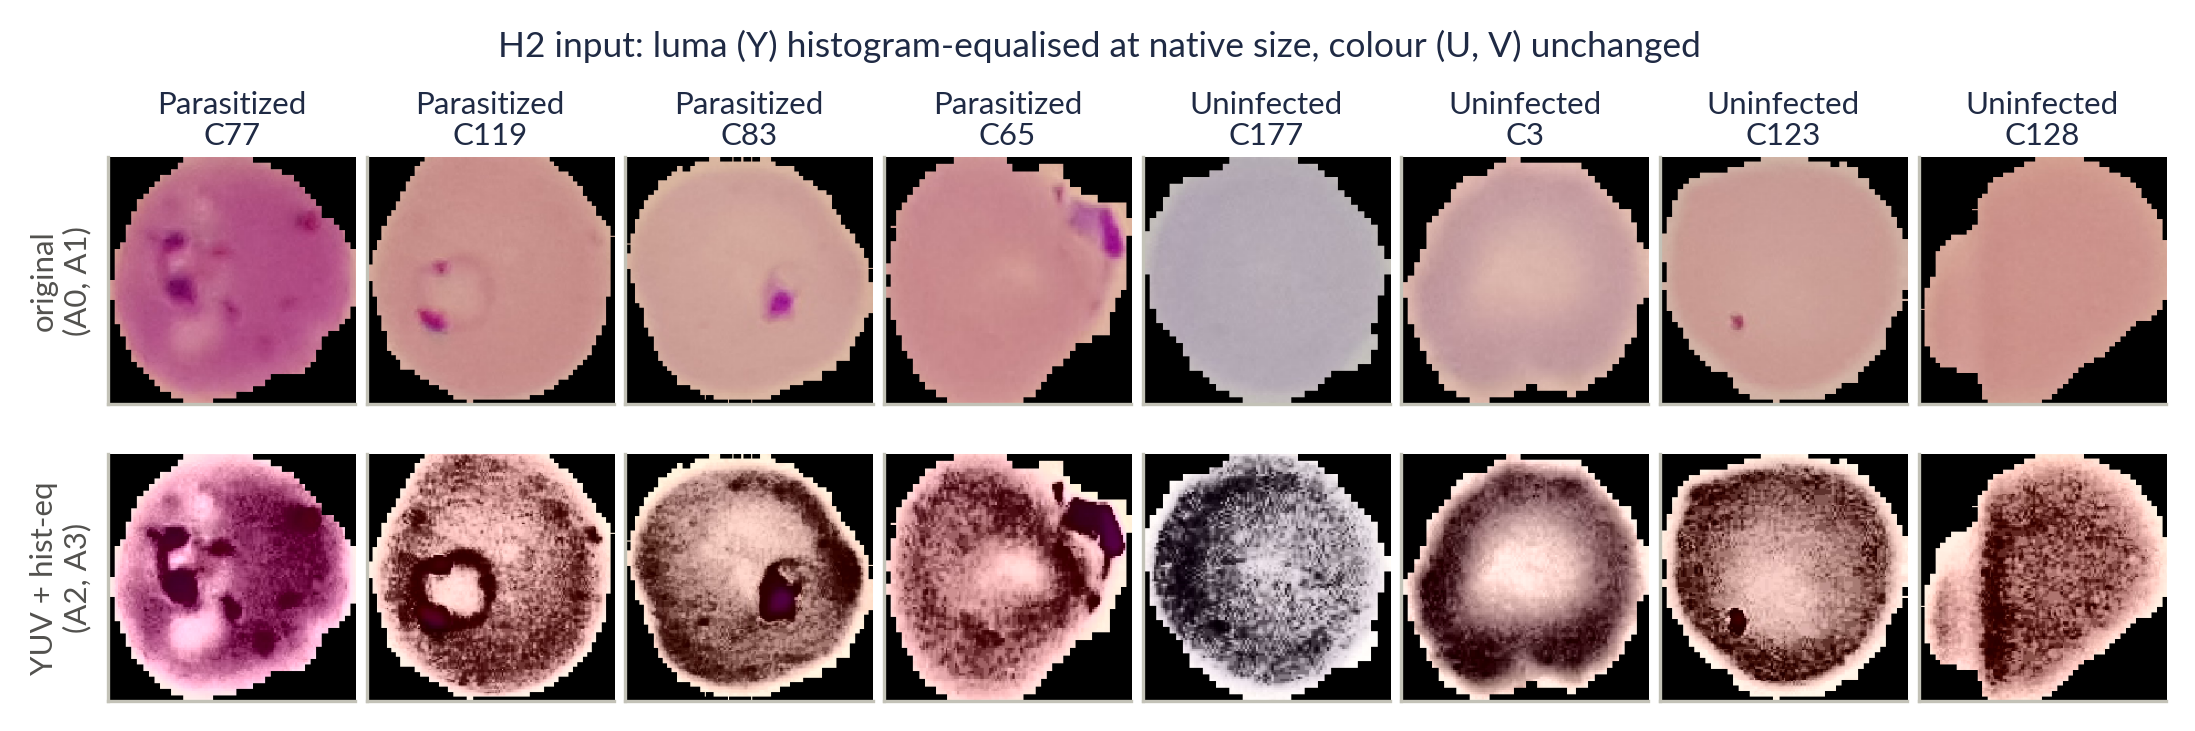
\includegraphics[width=\textwidth]{A2_yuv_slide/yuv_examples.png}
\caption{Input to H2. Top: original cells from eight different patients. Bottom: after YUV conversion and luma histogram equalisation.}
\label{fig:yuv}
\end{figure*}

\subsection{Statistical analysis}
All decisions below were committed to the repository before the A1, A2 and A3 models were trained. Patients are the unit of independence, so every confidence interval comes from a cluster bootstrap that resamples whole patients (\num{10000} resamples). The primary metric is the Matthews correlation coefficient (MCC), which is insensitive to the class mix that varies between patient folds; accuracy, recall (sensitivity for parasitized cells), specificity, balanced accuracy, $F_2$ and ROC-AUC are reported as well. The primary protocol evaluates clean (un-augmented) images; the paper's augmented protocol is reported alongside. Paired contrasts (A2 vs A1, A3 vs A0) use the corrected resampled $t$-test of Nadeau and Bengio~\cite{nadeau2003} on the ten per-fold differences, and a paired patient bootstrap of the ensemble's hold-out difference. A plain paired $t$-test would be too optimistic, because the folds' training sets overlap by about 89\,\%. A1 and A0 have different hold-out sets, so their ensembles are compared with independent patient bootstraps, and their folds with a Welch-type $t$-test in which each arm's variance carries the same correction. (Our plan specified a plain Welch test here; because it treats each arm's folds as independent, we apply the correction and report both.) $p$-values are Holm-corrected over the three contrasts~\cite{holm1979}. The decision rules restate the hypotheses as registered in our Phase~2 plan: H1 is supported if A1's ensemble MCC is lower than A0's with a 95\,\% interval excluding zero; H2 is rejected if A2's mean fold-MCC gain over A1 is smaller than A1's fold-to-fold standard deviation; the control shows ``little change'' if $|$A3$-$A0$|$ is below A0's fold standard deviation.

\textbf{Exploratory analyses.} After the results, a dated addendum fixed four further analyses before any of them was run:
\begin{itemize}
\item \emph{Equivalence.} Two one-sided tests~\cite{lakens2017} check equivalence within $\pm$1\,pp of MCC for the YUV contrasts, and we report each contrast's minimum detectable effect at 80\,\% power.
\item \emph{Leakage on identical cells.} A0's and A1's ensembles are scored on the \num{1095} A0 hold-out cells that belong to A1's 40 held-out patients. The two cross-validations' out-of-fold predictions are compared on the \num{17591} cells both contain. Each A0 model had seen other cells of the patient; no A1 model had.
\item \emph{Patient-level diagnosis.} A rule calls a patient positive if at least $\tau$ cells reach $P(\text{parasitized})\ge t$. It is chosen on the 160 cross-validation patients (highest Youden $J$ with at least 95\,\% specificity) and applied once to the 40 held-out patients.
\item \emph{Failure analysis.} We test whether errors cluster by patient, compare false-alarm rates in infected and healthy patients' smears, and flag candidate label errors by confident learning~\cite{northcutt2021}.
\end{itemize}

\begin{figure*}[t]
\centering
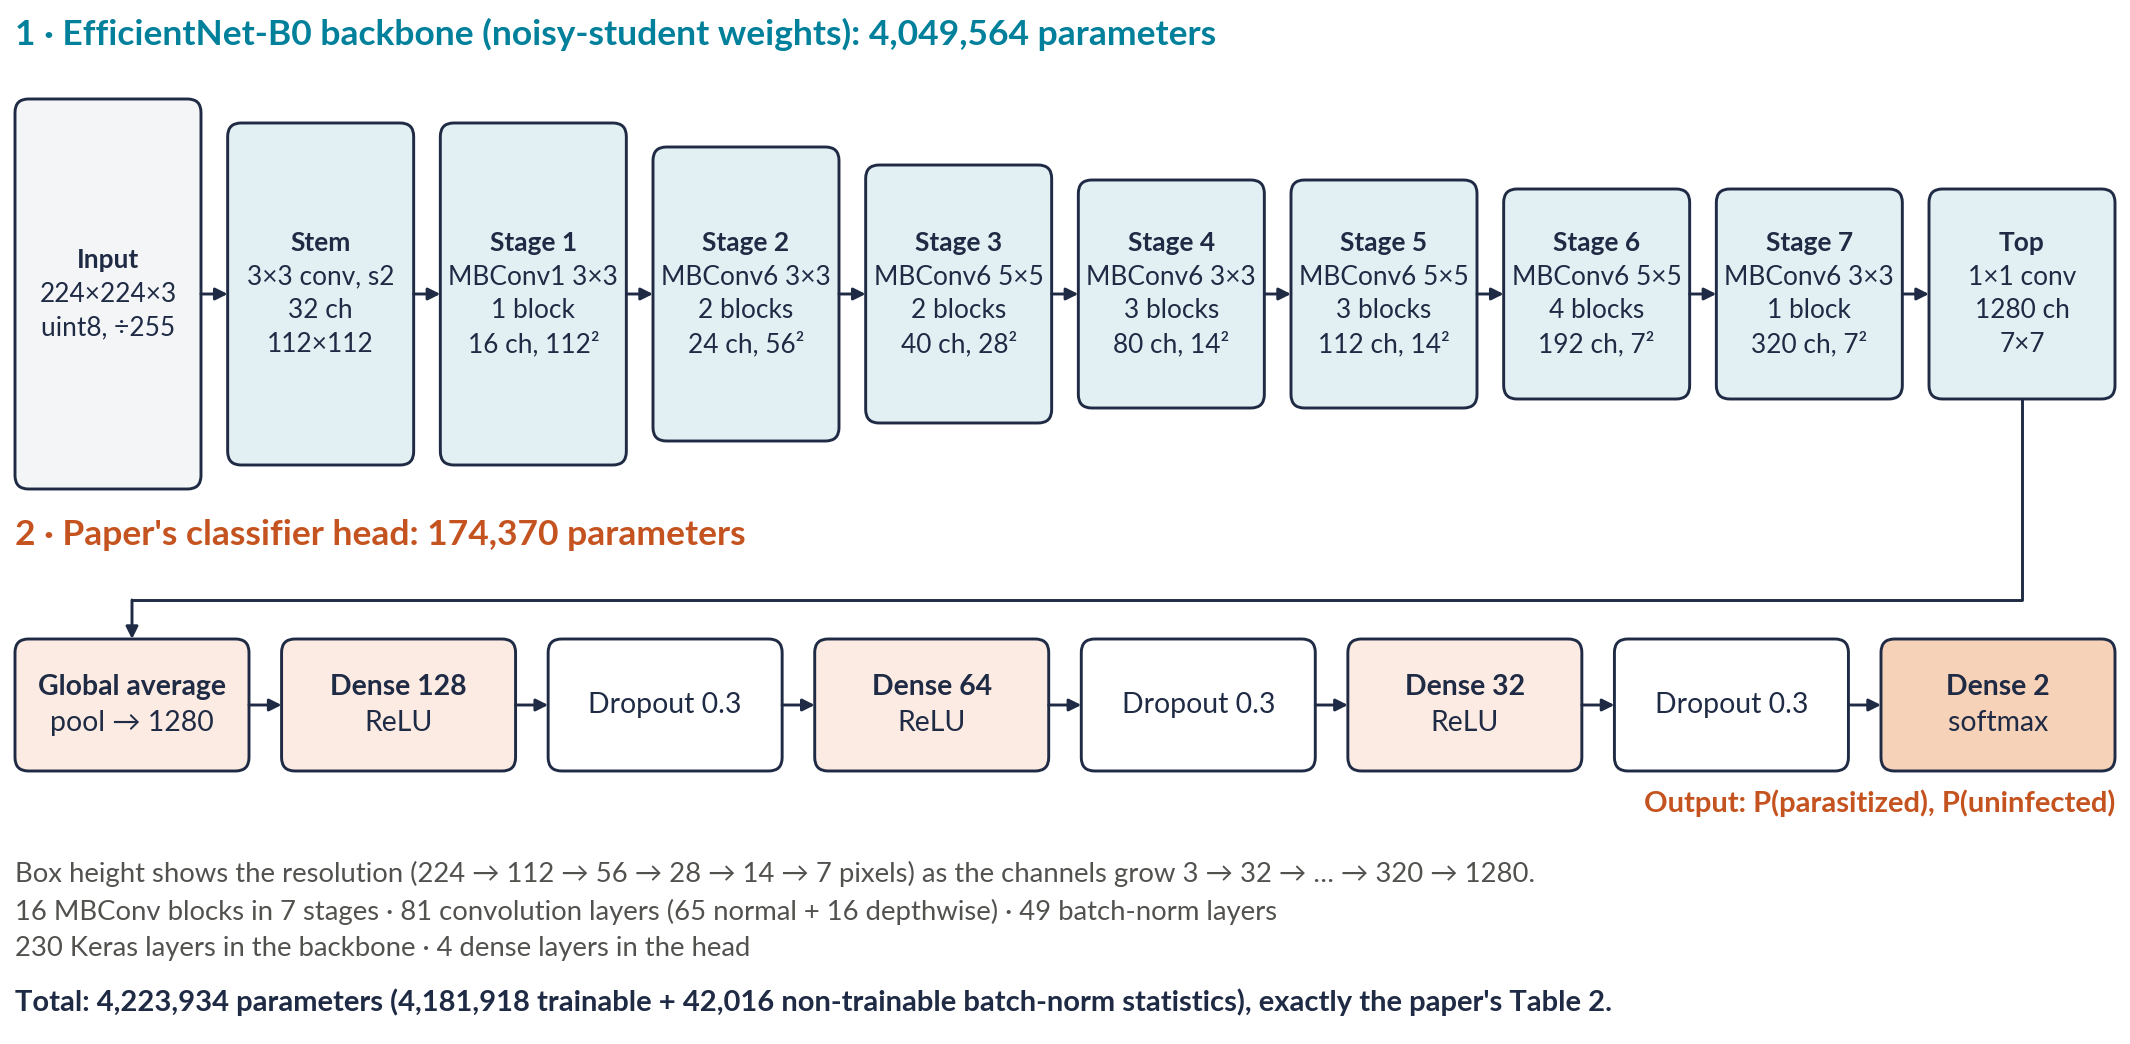
\includegraphics[width=\textwidth]{architecture.png}
\caption{The reproduced model: noisy-student EfficientNet-B0 (stem, 16 MBConv blocks in seven stages, $1\times1$ top convolution) and the paper's dense head. 4{,}223{,}934 parameters, exactly the paper's Table~2.}
\label{fig:arch}
\end{figure*}

% Generated by docs/ieee/make_tables.py from results/: do not edit by hand.
\begin{table}[t]
\centering
\caption{Reproduction of~\cite{marques2022} on the 5{,}512-cell hold-out set (\%). ``Paper protocol'' scores augmented images, as the authors' code did; ``clean'' scores the original images.}
\label{tab:repro}
\footnotesize
\setlength{\tabcolsep}{4pt}
\begin{tabular}{@{}lrrrr@{}}
\toprule
Metric & Paper & Ours (paper) & Ours (clean) & $\Delta$ \\
\midrule
Mean fold accuracy & 97.56 & 97.55 & 97.78 & $-$0.01 \\
Ensemble accuracy & 98.29 & 97.62 & 97.64 & $-$0.67 \\
Ensemble recall & 97.74 & 97.07 & 97.18 & $-$0.67 \\
Ensemble precision & 98.82 & 98.11 & 98.04 & $-$0.71 \\
Ensemble specificity & 98.84 & 98.17 & 98.09 & $-$0.67 \\
Ensemble F1 & 98.28 & 97.59 & 97.61 & $-$0.69 \\
Ensemble ROC-AUC & 99.76 & 99.73 & 99.68 & $-$0.03 \\
\bottomrule
\end{tabular}
\end{table}

\begin{table*}[t]
\centering
\caption{Ablation results, clean evaluation (\%). Folds: mean $\pm$ SD over the ten cross-validation test parts. Ensemble: the ten-model ensemble on each hold-out set, with 95\,\% patient-bootstrap intervals below each value. MCC $\times$100.}
\label{tab:ablation}
\footnotesize
\setlength{\tabcolsep}{4pt}
\resizebox{\ifdim\width>\textwidth\textwidth\else\width\fi}{!}{%
\begin{tabular}{@{}lllrrcccccc@{}}
\toprule
 & & & \multicolumn{2}{c}{Hold-out set} & \multicolumn{2}{c}{Folds, mean $\pm$ SD} & \multicolumn{4}{c}{Ensemble on the hold-out set [95\,\% CI]} \\
\cmidrule(lr){4-5} \cmidrule(lr){6-7} \cmidrule(l){8-11}
ID & Split & Prep. & Cells & Patients & MCC & Accuracy & Accuracy & MCC & Recall & ROC-AUC \\
\midrule
A0 & image & none & 5{,}512 & 200 & 95.57 $\pm$ 0.60 & 97.78 $\pm$ 0.30 & 97.64 & 95.29 & 97.18 & 99.68 \\
 & & & & & & & {\scriptsize [97.02, 98.17]} & {\scriptsize [94.03, 96.32]} & {\scriptsize [96.03, 98.06]} & {\scriptsize [99.52, 99.80]} \\[3pt]
A1 & patient & none & 5{,}550 & 40 & 93.92 $\pm$ 1.51 & 97.24 $\pm$ 0.66 & 98.45 & 96.90 & 98.05 & 99.80 \\
 & & & & & & & {\scriptsize [97.94, 98.91]} & {\scriptsize [95.70, 97.79]} & {\scriptsize [96.79, 98.85]} & {\scriptsize [99.61, 99.92]} \\[3pt]
A2 & patient & YUV & 5{,}550 & 40 & 93.32 $\pm$ 1.66 & 96.96 $\pm$ 0.75 & 98.32 & 96.65 & 98.22 & 99.76 \\
 & & & & & & & {\scriptsize [97.71, 98.86]} & {\scriptsize [95.23, 97.68]} & {\scriptsize [97.02, 99.02]} & {\scriptsize [99.55, 99.91]} \\[3pt]
A3 & image & YUV & 5{,}512 & 200 & 95.20 $\pm$ 0.37 & 97.60 $\pm$ 0.19 & 97.64 & 95.29 & 97.14 & 99.66 \\
 & & & & & & & {\scriptsize [97.02, 98.17]} & {\scriptsize [94.04, 96.32]} & {\scriptsize [95.94, 98.05]} & {\scriptsize [99.48, 99.79]} \\
\bottomrule
\end{tabular}}
\end{table*}

\begin{table*}[t]
\centering
\caption{Contrasts (new $-$ reference, percentage points). Fold: mean difference over the ten folds with 95\,\% CI (the corrected resampled $t$ of Nadeau and Bengio; for the unpaired H1 contrast, a Welch-type $t$ with the correction applied to each arm). Ensemble: hold-out difference with 95\,\% patient-bootstrap CI. $p$-values Holm-corrected over the three contrasts.}
\label{tab:contrasts}
\begin{tabular}{@{}llrrrr@{}}
\toprule
Contrast & Metric & Fold $\Delta$ [95\,\% CI] & Fold $p_{\mathrm{Holm}}$ & Ensemble $\Delta$ [95\,\% CI] & Ens. $p_{\mathrm{Holm}}$ \\
\midrule
H1: A1 $-$ A0 (unpaired) & MCC & $-$1.65 [$-$3.28, $-$0.02] & 0.142 & +1.62 [+0.01, +3.12] & 0.146 \\
 & Accuracy & $-$0.54 [$-$1.27, +0.18] & 0.364 & +0.81 [+0.06, +1.57] & 0.102 \\
 & Recall & $-$1.27 [$-$2.71, +0.18] & 0.240 & +0.87 [$-$0.67, +2.25] & 0.748 \\
 & Specificity & $-$0.26 [$-$1.10, +0.57] & 0.687 & +0.77 [+0.00, +1.53] & 0.118 \\
 & ROC-AUC & $-$0.23 [$-$0.54, +0.08] & 0.180 & +0.12 [$-$0.10, +0.32] & 0.593 \\
\midrule
H2: A2 $-$ A1 (paired) & MCC & $-$0.60 [$-$1.43, +0.22] & 0.246 & $-$0.26 [$-$0.85, +0.23] & 0.637 \\
 & Accuracy & $-$0.28 [$-$0.67, +0.11] & 0.364 & $-$0.13 [$-$0.41, +0.11] & 0.756 \\
 & Recall & $-$0.20 [$-$0.61, +0.21] & 0.609 & +0.18 [$-$0.11, +0.53] & 0.748 \\
 & Specificity & $-$0.33 [$-$0.91, +0.25] & 0.687 & $-$0.44 [$-$0.92, $-$0.04] & 0.118 \\
 & ROC-AUC & $-$0.18 [$-$0.39, +0.02] & 0.180 & $-$0.04 [$-$0.09, +0.02] & 0.593 \\
\midrule
Control: A3 $-$ A0 (paired) & MCC & $-$0.37 [$-$0.87, +0.12] & 0.246 & +0.00 [$-$0.52, +0.53] & 1.000 \\
 & Accuracy & $-$0.19 [$-$0.43, +0.06] & 0.364 & +0.00 [$-$0.26, +0.27] & 1.000 \\
 & Recall & $-$0.10 [$-$0.43, +0.23] & 0.609 & $-$0.04 [$-$0.43, +0.33] & 0.935 \\
 & Specificity & $-$0.27 [$-$0.85, +0.30] & 0.687 & +0.04 [$-$0.36, +0.43] & 0.917 \\
 & ROC-AUC & $-$0.16 [$-$0.33, +0.01] & 0.180 & $-$0.02 [$-$0.11, +0.05] & 0.663 \\
\bottomrule
\end{tabular}
\end{table*}

\begin{table}[t]
\centering
\caption{Recall-first threshold (best $F_2$ on the cross-validation predictions, applied once to the hold-out set) and expected calibration error (ECE). Clean evaluation, \%.}
\label{tab:extras}
\footnotesize
\setlength{\tabcolsep}{4pt}
\begin{tabular}{@{}lrrrrr@{}}
\toprule
 & & \multicolumn{2}{c}{Recall} & Specificity & \\
\cmidrule(lr){3-4}
ID & Threshold & at 0.5 & at threshold & at threshold & ECE \\
\midrule
A0 & 0.192 & 97.18 & 98.72 & 95.22 & 0.053 \\
A1 & 0.189 & 98.05 & 99.22 & 93.93 & 0.065 \\
A2 & 0.143 & 98.22 & 99.22 & 91.74 & 0.060 \\
A3 & 0.159 & 97.14 & 98.75 & 94.14 & 0.052 \\
\bottomrule
\end{tabular}
\end{table}

\begin{table}[t]
\centering
\caption{Exploratory analyses, fixed in a dated addendum before they were run. Clean evaluation. The leakage rows score 1{,}095 hold-out and 17{,}591 cross-validation cells; H2 is A2 $-$ A1, the control A3 $-$ A0.}
\label{tab:phase3b}
\footnotesize
\setlength{\tabcolsep}{4pt}
\begin{tabular}{@{}lrrc@{}}
\toprule
 & & & Within \\
Analysis & Estimate & Interval & $\pm$1\,pp? \\
\midrule
\multicolumn{4}{@{}l}{\textit{Leakage on identical cells: A1 $-$ A0, MCC (pp), 95\,\% CI}} \\
\quad Ensembles, 40 patients & +0.00 & [$-$0.90, +0.98] & \\
\quad Out-of-fold, 160 patients & $-$0.85 & [$-$2.02, $-$0.05] & \\
\addlinespace
\multicolumn{4}{@{}l}{\textit{YUV effect: MCC (pp), 90\,\% CI}} \\
\quad H2, ensembles & $-$0.26 & [$-$0.73, +0.16] & yes \\
\quad H2, folds & $-$0.60 & [$-$1.27, +0.06] & no \\
\quad Control, ensembles & +0.00 & [$-$0.44, +0.44] & yes \\
\quad Control, folds & $-$0.37 & [$-$0.77, +0.03] & yes \\
\addlinespace
\multicolumn{4}{@{}l}{\textit{Patient level: 40 held-out patients, \%, exact 95\,\% CI}} \\
\quad Sensitivity, 26/28 & 92.9 & [76.5, 99.1] & \\
\quad Specificity, 12/12 & 100.0 & [73.5, 100.0] & \\
\bottomrule
\end{tabular}
\end{table}



\section{Results}
\subsection{Reproduction within 1\,pp, 25 times faster}
Table~\ref{tab:repro} compares our ten-fold reproduction with the outputs printed by the authors' code. The fold models match the paper to 0.01\,pp (97.55 vs.\ 97.56\,\% mean accuracy on their cross-validation test parts), and every headline metric is within 1\,pp. The ensemble lands within 0.67\,pp of the paper's 98.29\,\%, about three standard errors of a \num{5512}-cell test set: it gains 0.25\,pp over its average member where the paper's gained 0.60\,pp, and the paper's unseeded split and the newer TensorFlow are the remaining differences. Scoring clean instead of augmented images changes our numbers by at most 0.23\,pp, so the paper's augmented evaluation does not explain its results. Reading the authors' code also exposed reporting errors: the paper's text swaps the ensemble's precision and recall (the true recall is 97.74\,\%, not 98.82\,\%), and its Table~6 ``accuracy'' is $(\text{precision}+\text{recall})/2$ of each report.

\subsection{H1: accuracy holds on unseen patients}
Table~\ref{tab:ablation} lists all four experiments and Table~\ref{tab:contrasts} the three contrasts. On the 40 held-out patients, the A1 ensemble reaches \textbf{98.45\,\%} accuracy (95\,\% CI 97.94 to 98.91), 98.05\,\% recall, 99.80\,\% ROC-AUC and an MCC of 96.90, on par with A0's 97.64\,\% on its image-split hold-out set (MCC difference $+1.62$\,pp, 95\,\% CI $+0.01$ to $+3.12$, Holm $p=0.15$). By the pre-registered rule, H1 is not supported: the paper's accuracy holds on patients the model has never seen.

Cross-validation over the other 160 patients confirms the second half of H1's prediction (Fig.~\ref{fig:folds}): the fold-to-fold spread widens 2.5-fold (MCC SD 0.60 to 1.51), the signature of genuine patient-to-patient variation. The mean fold MCC moves from 95.57 to 93.92 ($-1.65$\,pp, 95\,\% CI $-3.28$ to $-0.02$, Holm $p=0.14$) and the mean fold accuracy from 97.78 to 97.24\,\%; the uncorrected Welch test of our plan gave $p=0.0075$ (Holm 0.023). The same A1 models score 98.22\,\% on the 40 held-out patients and 97.24\,\% in cross-validation, so this hold-out draw is about 1\,pp easier than an average group of unseen patients, a lesson we return to in Section~\ref{sec:discussion}. Validation on unseen patients also peaks earlier: the best epoch falls at a median of 17 instead of 28.5.

\textbf{Leakage measured on identical cells.} The two comparisons above score different cells, and the unpaired hold-out comparison could detect only about 2.2\,pp of MCC with 80\,\% power. Scoring the same cells with both arms isolates patient leakage (Fig.~\ref{fig:leakage}, Table~\ref{tab:phase3b}):
\begin{itemize}
\item On the \num{17591} cross-validation cells both arms share, A1's out-of-fold models score 0.85\,pp lower in MCC than A0's (95\,\% CI 0.05 to 2.02; accuracy $-0.43$\,pp).
\item On the \num{1095} A0 hold-out cells of A1's 40 held-out patients, the two ensembles have identical confusion matrices (difference 0.00\,pp, 95\,\% CI $-0.90$ to $+0.98$), and 19 of each ensemble's 22 errors fall on the same cells.
\end{itemize}
Patient leakage is therefore measurable but small on this dataset. A0's models also trained on more patients, so these differences, if anything, overstate it.

\begin{figure*}[t]
\centering
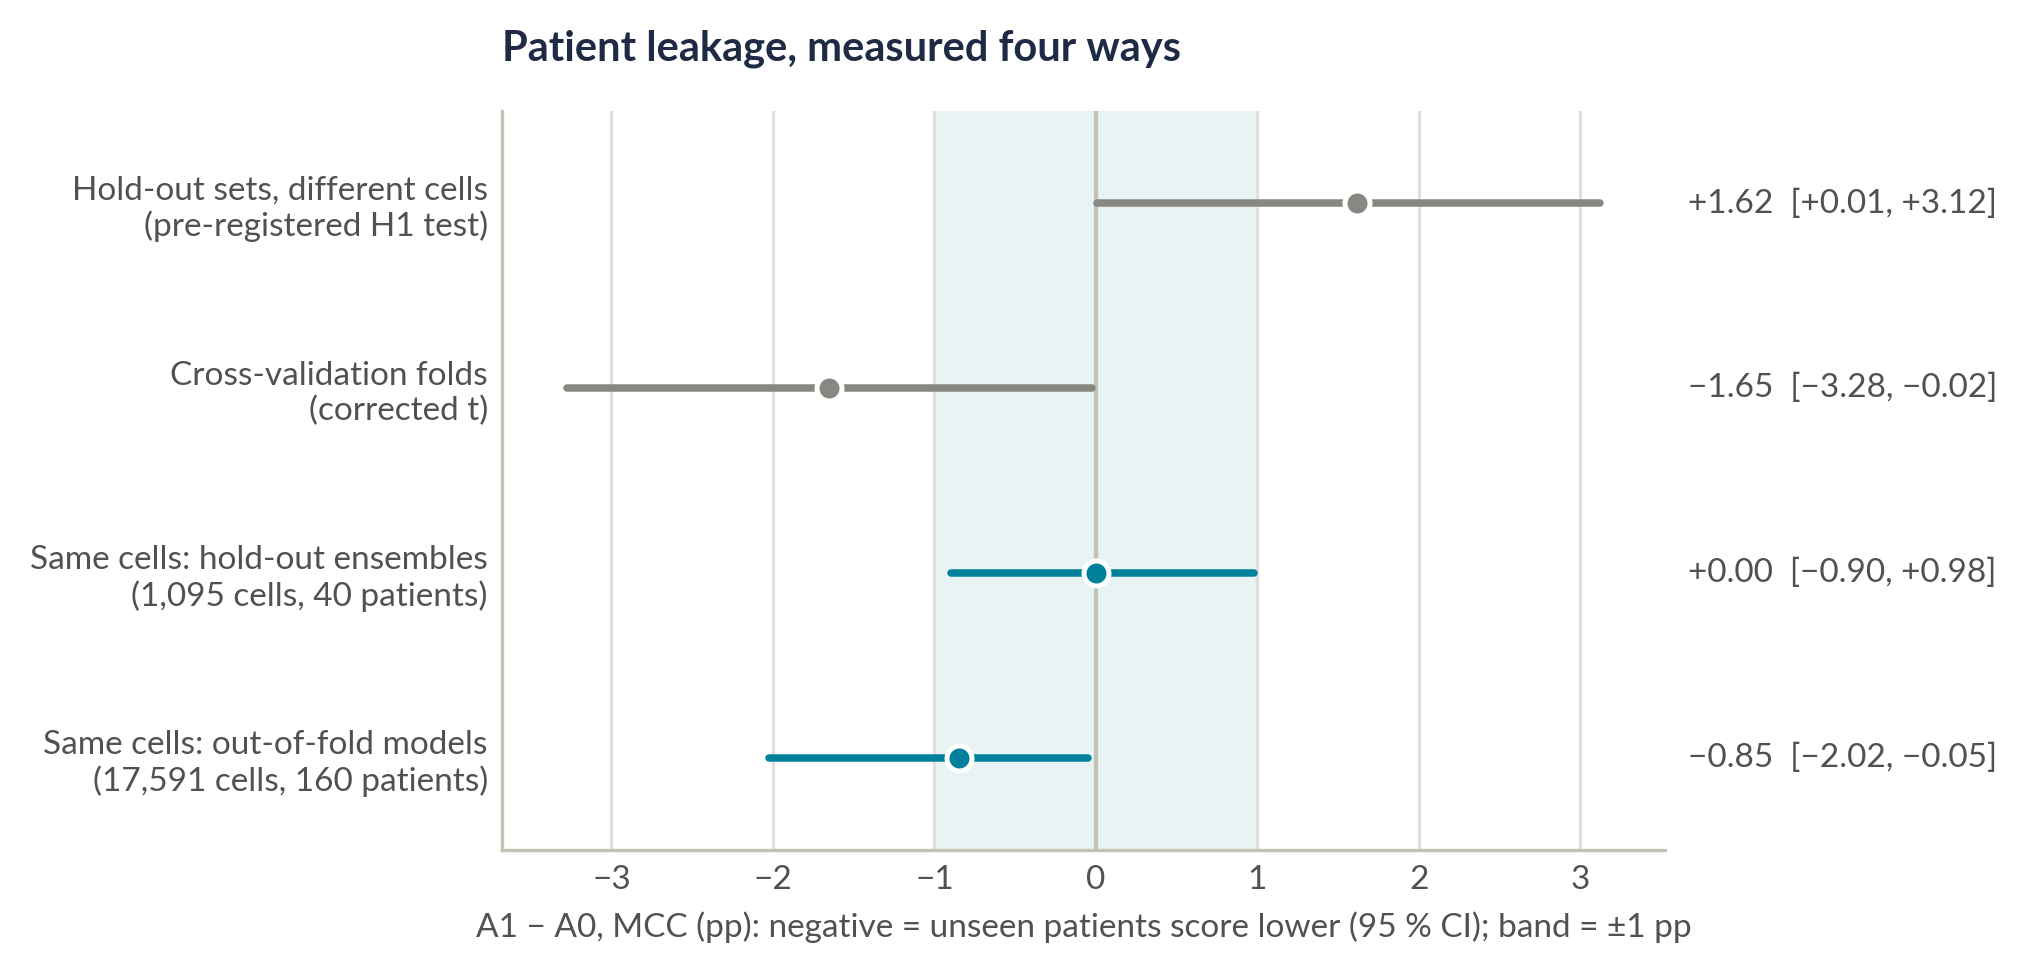
\includegraphics[width=0.85\textwidth]{phase3b/phase3b_leakage.png}
\caption{A1 $-$ A0 in MCC, measured four ways (95\,\% CIs; shaded: $\pm$1\,pp). The pre-registered hold-out comparison scores different cells; the cross-validation folds use the corrected $t$-test; the two teal rows score identical cells and isolate patient leakage.}
\label{fig:leakage}
\end{figure*}

\begin{figure*}[t]
\centering
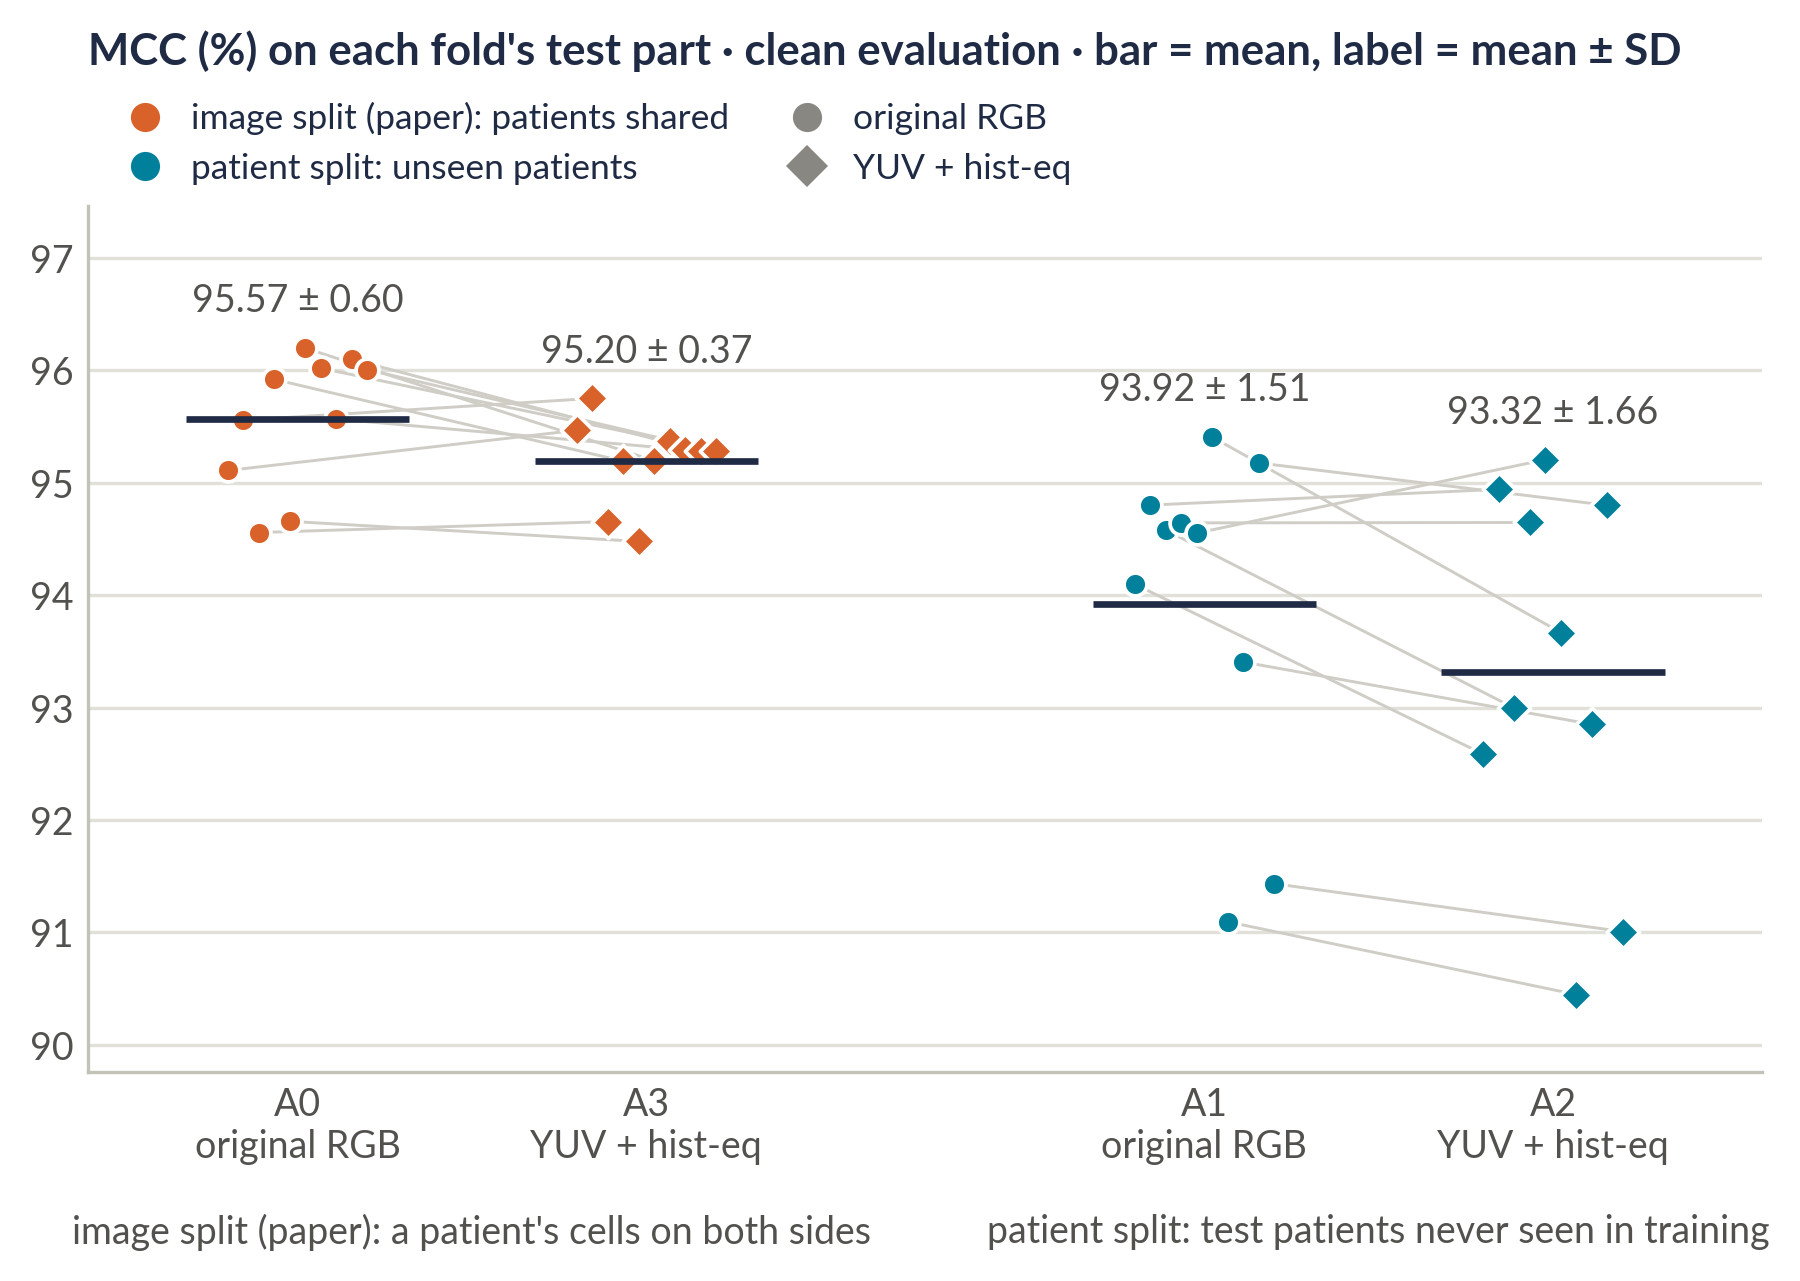
\includegraphics[width=0.82\textwidth]{ablation/ablation_fold_mcc.png}
\caption{MCC of every fold model on its cross-validation test part (clean evaluation). Orange: the paper's image split; teal: the patient split. Grey lines join the same fold across the paired YUV change. Patient-split folds vary 2.5 times more, as H1 predicted, with a mean 1.65\,pp lower; YUV changes little.}
\label{fig:folds}
\end{figure*}

\begin{figure*}[t]
\centering
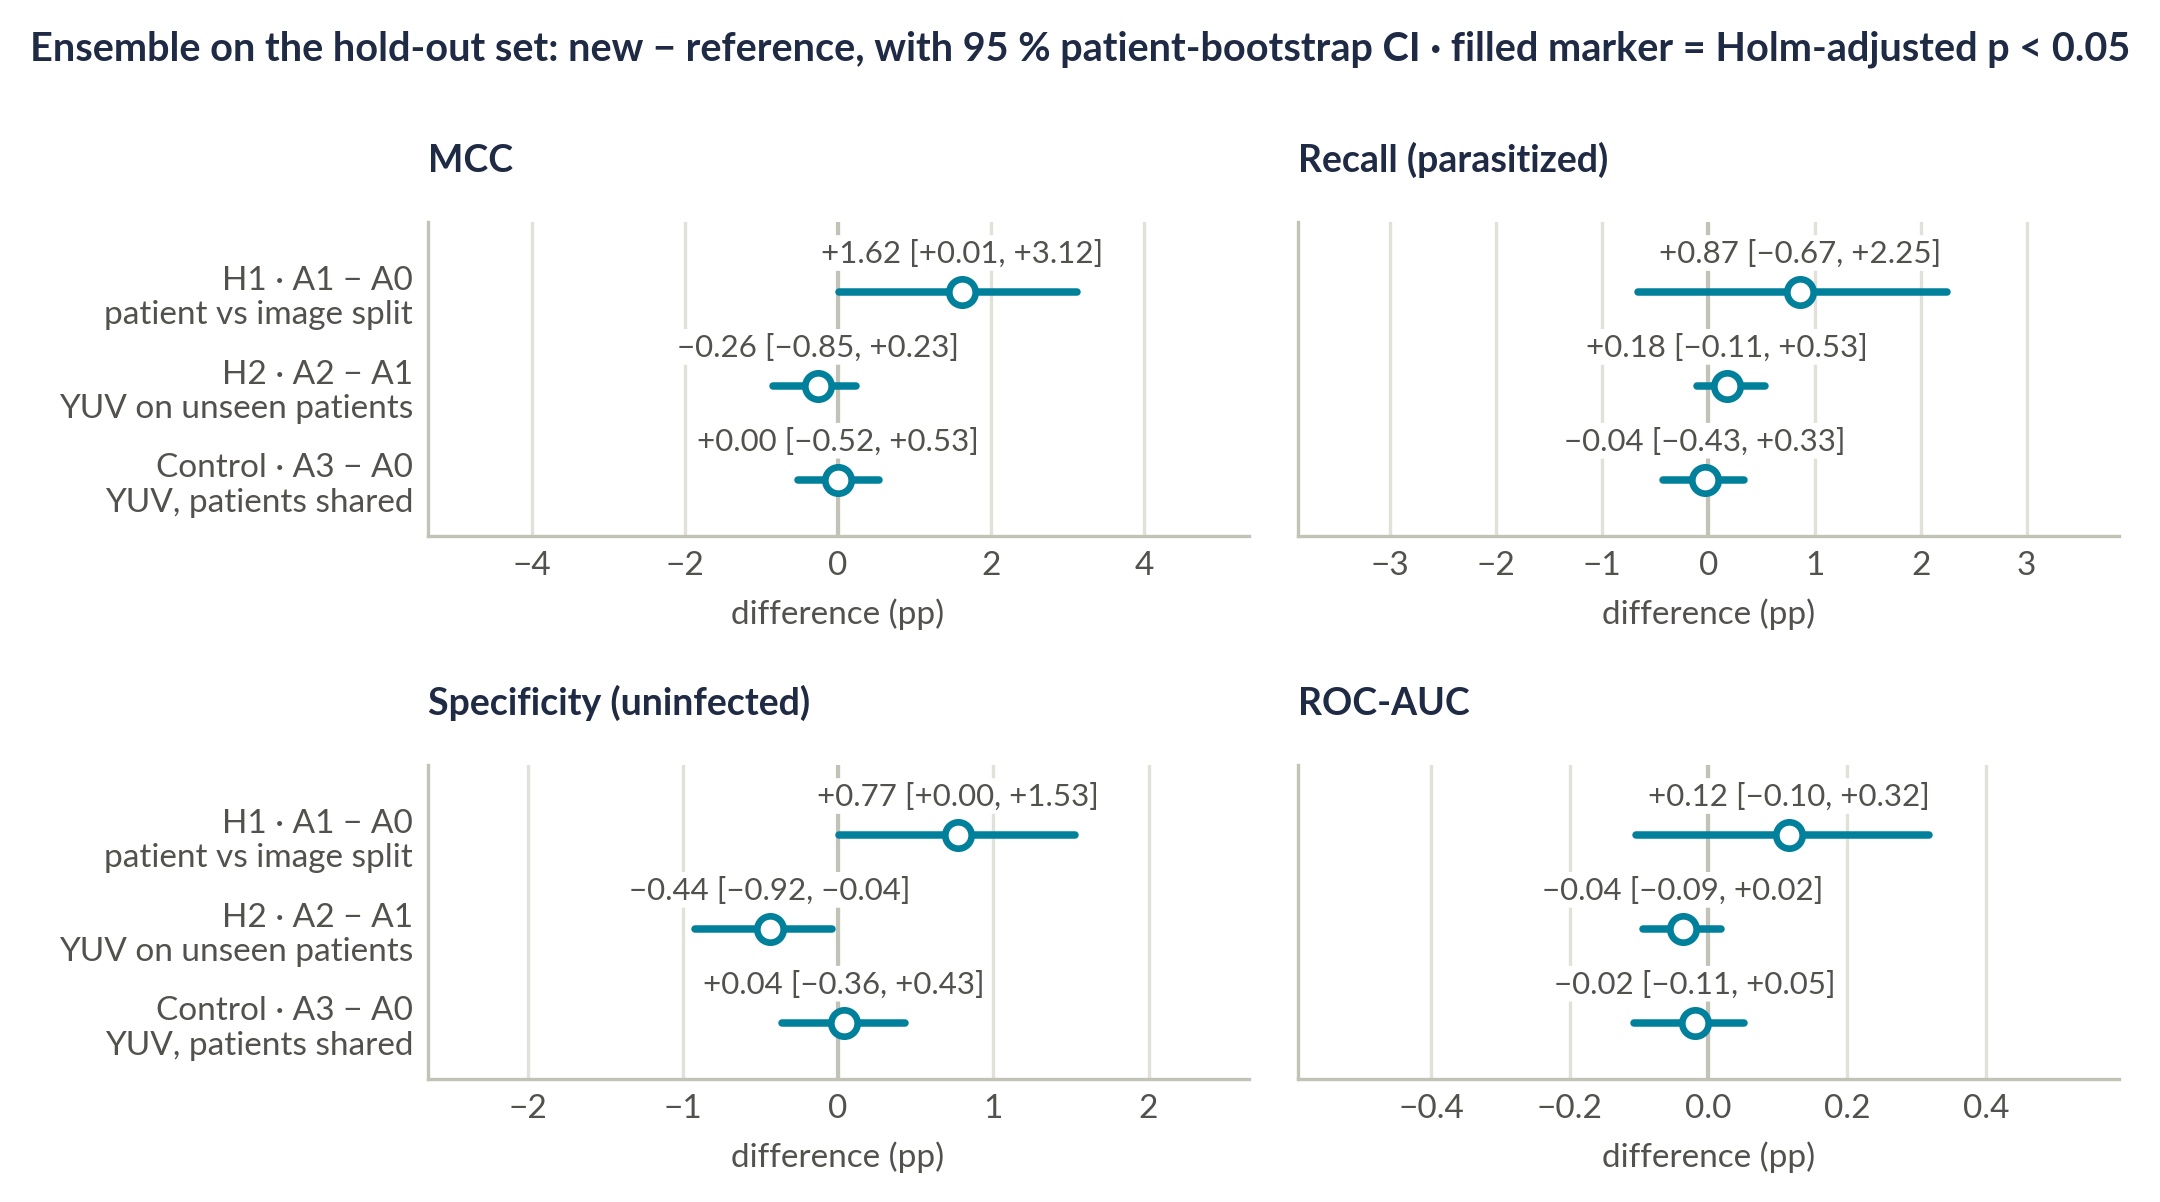
\includegraphics[width=\textwidth]{ablation/ablation_contrasts_2x2.png}
\caption{The three contrasts on the ensembles' hold-out sets, with 95\,\% patient-bootstrap intervals. After Holm correction, neither the patient split nor YUV changes any metric significantly.}
\label{fig:contrasts}
\end{figure*}

\subsection{H2: the model is already stain-robust}
On the same unseen patients, adding YUV normalisation (A2 vs.\ A1) changes the mean fold MCC by $-0.60$\,pp, less than A1's fold-to-fold standard deviation of 1.51\,pp, so the pre-registered rule rejects H2; the corrected resampled $t$-test agrees ($p=0.13$). On the hold-out set the ensemble MCC changes by $-0.26$\,pp (95\,\% CI $-0.85$ to $+0.23$); recall holds ($+0.18$\,pp) and specificity moves by $-0.44$\,pp, not significant after correction (Fig.~\ref{fig:contrasts}). The control A3 vs.\ A0 shows no detectable effect when patients are shared (ensemble MCC $+0.00$\,pp, 95\,\% CI $-0.52$ to $+0.53$). The analysis under the paper's augmented protocol gives the same three verdicts.

Equivalence tests bound the effect (Table~\ref{tab:phase3b}).
\begin{itemize}
\item On the hold-out set, YUV changes MCC by $-0.73$ to $+0.16$\,pp (90\,\% CI): inside a $\pm$1\,pp margin (TOST $p=0.008$) and below the 0.77\,pp this paired design can detect. The baseline is already robust to the brightness variation YUV removes, so the simpler pipeline loses nothing.
\item At the fold level the interval ($-1.27$ to $+0.06$) is too wide to establish equivalence.
\item The control is equivalent within $\pm$1\,pp at both levels.
\end{itemize}

\subsection{Screening operating point}
For screening, a missed infected cell is costlier than a false alarm. Choosing the decision threshold on the pooled out-of-fold cross-validation predictions (maximum $F_2$) and applying it once to the hold-out set lifts recall to 98.7 to 99.2\,\% at a specificity of 91.7 to 95.2\,\% (Table~\ref{tab:extras}); for A1, from 98.05 to 99.22\,\%. The ensembles rank cells almost perfectly (ROC-AUC 99.66 to 99.80\,\%) and are slightly under-confident (ECE 0.05 to 0.07), as the paper's label smoothing predicts.

\subsection{Patient-level diagnosis (exploratory)}
The rule chosen on the 160 cross-validation patients' out-of-fold predictions calls a patient positive if \emph{at least 3 cells have $P(\text{parasitized})\ge0.80$}. On those patients its sensitivity is 96.7\,\% and its specificity 100\,\%; selecting the rule in a nested leave-one-fold-out gives 96.7\,\% and 97.4\,\%. Applied once to the 40 held-out patients with the A1 ensemble, it identifies 26 of 28 infected patients (92.9\,\%, exact 95\,\% CI 76.5 to 99.1) and clears all 12 healthy ones (100\,\%, 73.5 to 100).

The two missed patients, C53 and C73, are the only held-out patients with just three parasitized crops. When each infected patient keeps only one or two parasitized crops, sensitivity falls to 3.6 and 12.3\,\%. NIH kept about 68 uninfected crops per patient but curated the parasitized ones, so these numbers describe aggregation on curated crops, not diagnostic accuracy on a smear.

\subsection{Failure analysis (exploratory)}
\begin{itemize}
\item \emph{Errors cluster by patient} (permutation test $p<0.001$): half of A1's 86 hold-out errors come from 7 of the 40 patients, and 14 patients have none.
\item \emph{False alarms concentrate in infected patients' smears.} The model flags 1.57\,\% of their uninfected-labelled cells, against 0.12\,\% in healthy patients (difference 1.45\,pp, 95\,\% CI 0.82 to 2.14); out of fold the rates are 2.35 and 0.85\,\%. This fits parasites missed in the labels, or genuinely ambiguous cells next to parasites; separating the two needs an expert, and a blind triage protocol for it is published with our code.
\item \emph{Candidate label errors.} Confident learning flags 8 hold-out cells. Removing them leaves both YUV contrasts unchanged.
\end{itemize}

\subsection{Compute}
Each of the 40 models trains for 33 epochs in about 11 minutes on an RTX~4090 (10.2 to 12.8 minutes for A1 to A3) and in 11 to 18 minutes on an L40S, against 4\,h\,46\,min per fold reported for a GTX~1050. A1 to A3 ran as one cloud pod per fold that trains the three experiments in turn: 30 models in about one hour of wall-clock time for US\$6.95.

\section{Discussion}
\label{sec:discussion}
\textbf{Why the model generalises across patients.} Rajaraman \emph{et al.}~\cite{rajaraman2018} reported a drop from 98.6 to 95.9\,\% when moving from cell-level to patient-level evaluation with features from pre-trained networks. Our end-to-end fine-tuned ensemble loses about half a point of accuracy: 0.43\,pp on identical cells (0.85\,pp of MCC) and 0.54\,pp in cross-validation. Methods and protocols differ, so the comparison is indicative, but a fully fine-tuned, heavily augmented network appears to lean far less on patient identity. Two plausible reasons, which our experiments do not separate, are that the decisive cue (stained parasite chromatin) looks alike across patients, and that the paper's heavy colour, contrast and blur augmentation already prevents the network from relying on a patient's staining.

\textbf{Evaluate on several patient groups.} The 40-patient hold-out set is about 1\,pp easier than an average fold of unseen patients. That is larger than the leakage effect and larger than the paper's own margins over competing methods. Patient clustering also inflates the variance of hold-out accuracy 2.3-fold (MCC 2.6-fold) compared with treating cells as independent. Sub-1-pp differences between published methods therefore cannot be resolved on a single random hold-out set. The standard we recommend, and apply here, is cross-validation over patients with patient-level confidence intervals, plus paired comparisons on identical cells where possible.

\textbf{Why stain normalisation is redundant here.} Umer \emph{et al.}~\cite{umer2020} reported 99.96\,\% with their full preprocessing against 49.61\,\% without it. That comparison is against a model that did not train, not against a strong baseline. With a pre-trained network and an augmentation pipeline that already randomises brightness and contrast (including CLAHE), explicit equalisation adds nothing. The step also changes luma only: it normalises brightness, not stain colour. In histopathology, colour augmentation rather than normalisation gave the most robust models across laboratories~\cite{tellez2019}, and the recipe here has none, so a colour-augmentation arm tested on another laboratory's smears is the natural next experiment. By stretching each cell's narrow luma range to the full scale (Fig.~\ref{fig:yuv}), the step also amplifies texture and noise, consistent with the small change in specificity we observe.

\section{Limitations}
The patient-level rule is exploratory: NIH curated the parasitized crops (and kept about 68 uninfected crops per patient), and only 12 held-out patients are healthy; evaluating the rule on whole smears is the next step. All data come from one hospital, so a patient split removes patient leakage but not site or staining-protocol effects, and H2 is tested on the same laboratory's stain; an external test set is the next step. Labels come from a single expert. Fuhad \emph{et al.}~\cite{fuhad2020} set aside 1{,}397 cells (5.1\,\%) as mislabelled or suspicious, but their list is no longer available, so we keep the original labels, as the paper did, and flag candidates for expert review. Each comparison rests on one hold-out draw and one training run per fold and arm; patient-bootstrap intervals and ten-fold cross-validation quantify that uncertainty, though the out-of-fold same-cell interval omits run-to-run noise. Within each fold, A1, A2 and A3 shared one GPU, so the paired comparisons use identical hardware.

\section{Conclusion}
Rebuilt exactly from its authors' code and trained about 25 times faster, the EfficientNet-B0 ensemble of Marques \emph{et al.} reproduces within 1\,pp on every metric, and a pre-registered, patient-level ablation shows that its accuracy holds on patients it has never seen: 98.45\,\% accuracy, 98.05\,\% recall and 99.80\,\% ROC-AUC on 40 held-out patients. Measured on identical cells, patient leakage is small (0.85\,pp of MCC), and YUV stain normalisation, reported as highly effective in the literature, is equivalent to no preprocessing within $\pm$1\,pp, so the simpler pipeline suffices. Combining cell calls per patient identifies 26 of 28 infected and all 12 healthy held-out patients on curated crops. Future work will test on an external laboratory's smears, triage the remaining errors blind against an independent relabelling, evaluate patient-level rules on whole smears, and distil the ensemble into a single model light enough for point-of-care use. Code, results, the analysis plan and all 40 trained models are public.


\begin{thebibliography}{99}
\bibitem{liang2016} Z.~Liang \emph{et al.}, ``CNN-based image analysis for malaria diagnosis,'' in \emph{Proc. IEEE Int. Conf. Bioinformatics and Biomedicine (BIBM)}, 2016.
\bibitem{rajaraman2018} S.~Rajaraman \emph{et al.}, ``Pre-trained convolutional neural networks as feature extractors toward improved malaria parasite detection in thin blood smear images,'' \emph{PeerJ}, vol.~6, p.~e4568, 2018.
\bibitem{rajaraman2019} S.~Rajaraman, S.~Jaeger, and S.~K. Antani, ``Performance evaluation of deep neural ensembles toward malaria parasite detection in thin-blood smear images,'' \emph{PeerJ}, vol.~7, p.~e6977, 2019.
\bibitem{umer2020} M.~Umer, S.~Sadiq, M.~Ahmad, S.~Ullah, G.~S. Choi, and A.~Mehmood, ``A novel stacked CNN for malarial parasite detection in thin blood smear images,'' \emph{IEEE Access}, vol.~8, 2020, doi: 10.1109/ACCESS.2020.2994810.
\bibitem{fuhad2020} K.~M.~F. Fuhad \emph{et al.}, ``Deep learning based automatic malaria parasite detection from blood smear and its smartphone based application,'' \emph{Diagnostics}, vol.~10, no.~5, p.~329, 2020.
\bibitem{zhao2020} O.~S. Zhao \emph{et al.}, ``Convolutional neural networks to automate the screening of malaria in low-resource countries,'' \emph{PeerJ}, vol.~8, p.~e9674, 2020.
\bibitem{masud2020} M.~Masud \emph{et al.}, ``Leveraging deep learning techniques for malaria parasite detection using mobile application,'' \emph{Wireless Commun. Mobile Comput.}, vol.~2020, p.~8895429, 2020.
\bibitem{marques2022} G.~Marques, A.~Ferreras, and I.~de~la Torre-D\'iez, ``An ensemble-based approach for automated medical diagnosis of malaria using EfficientNet,'' \emph{Multimedia Tools Appl.}, vol.~81, pp.~28061--28078, 2022, doi: 10.1007/s11042-022-12624-6.
\bibitem{madhu2023} G.~Madhu \emph{et al.}, ``Intelligent diagnostic model for malaria parasite detection and classification using imperative inception-based capsule neural networks,'' \emph{Sci. Rep.}, vol.~13, Art. no.~13377, 2023.
\bibitem{hemachandran2023} K.~Hemachandran \emph{et al.}, ``Performance analysis of deep learning algorithms in diagnosis of malaria disease,'' \emph{Diagnostics}, vol.~13, no.~3, p.~534, 2023.
\bibitem{mujahid2024} M.~Mujahid \emph{et al.}, ``Efficient deep learning-based approach for malaria detection using red blood cell smears,'' \emph{Sci. Rep.}, vol.~14, Art. no.~13249, 2024.
\bibitem{tan2019} M.~Tan and Q.~V. Le, ``EfficientNet: Rethinking model scaling for convolutional neural networks,'' in \emph{Proc. ICML}, 2019, pp.~6105--6114.
\bibitem{xie2020} Q.~Xie, M.-T. Luong, E.~Hovy, and Q.~V. Le, ``Self-training with noisy student improves ImageNet classification,'' in \emph{Proc. CVPR}, 2020, pp.~10687--10698.
\bibitem{nadeau2003} C.~Nadeau and Y.~Bengio, ``Inference for the generalization error,'' \emph{Mach. Learn.}, vol.~52, no.~3, pp.~239--281, 2003.
\bibitem{holm1979} S.~Holm, ``A simple sequentially rejective multiple test procedure,'' \emph{Scand. J. Statist.}, vol.~6, no.~2, pp.~65--70, 1979.
\bibitem{lakens2017} D.~Lakens, ``Equivalence tests: A practical primer for $t$ tests, correlations, and meta-analyses,'' \emph{Soc. Psychol. Personal. Sci.}, vol.~8, no.~4, pp.~355--362, 2017.
\bibitem{northcutt2021} C.~G. Northcutt, L.~Jiang, and I.~L. Chuang, ``Confident learning: Estimating uncertainty in dataset labels,'' \emph{J. Artif. Intell. Res.}, vol.~70, pp.~1373--1411, 2021.
\bibitem{tellez2019} D.~Tellez \emph{et al.}, ``Quantifying the effects of data augmentation and stain color normalization in convolutional neural networks for computational pathology,'' \emph{Med. Image Anal.}, vol.~58, Art. no.~101544, 2019.
\end{thebibliography}

\end{document}
